\chapter{Počítačové videnie}
\section{Úvod}
Počítačové videnie je vedná disciplína, ktorá sa snaží počítačovými prostriedkami napodobniť ľudské videnie. Základom je spracovanie 2D obrazu (Image Processing). Túto etapu väčšinou predstavujú algoritmy na nízkej úrovni abstrakcie (low-level). Algoritmy, ktoré extrahujú z nižšej úrovne znalosti, dávajú ich do súvislostí a snažia sa im porozumieť (Image understanding, machine learning) pracujú na vyššej úrovni (hight-level). To by nebolo možné bez znalosti fyzikálnej podstaty senzorov, optiky, okolitého prostredia a tiež matematických a štatistických metód na ich hodnotenie.

\section{Najvýznamnejšie problémy počítačového videnia}
\begin{itemize}
\item Strata informácie pri premietaní z 3D do 2D. Človek totiž vníma okolitý svet ako 3-rozmerný,však väčšina senzorov a snímacích zariadení je schopná registrovať iba 2D.
\item Interpretácia ľudského mozgu nieje správna. Sietnica ľudského oka je dvojrozmerná preto trojrozmernú predstavou okolia vytvára mozog, na základe znalostí.
\item Šum. Je prítomný v každom reálnom obraze. Preto namiesto deterministických modelov je potrebné používať stochastické modely, ktoré predpokladajú určitý stupeň neurčitosti a dokážu túto neurčitosť aj zahrnúť do matematického modelu.
\item Obrovský tok dát prijímaný zo snímačov obrazu, ktoré je nutné spracovať v reálnom čase.
\item Nejednoznačná interpretácia jasu jednotlivých častí objektu. Bez poznania fyzikálnej povahy sledovaného objektu nie sme schopní jednoznačne určiť, či výrazné svetlé škvrny na obraze sú dôsledkom extrémne svetlých častí objektu alebo iba dôsledkom odrazu zdroja svetla v lesklej (ale nie svetlej) časti povrchu.
\end{itemize}


\section{Etapy spracovania obrazu}

Jednotlivé etapy spracovávania obrazu možno vyjadriť grafom, ktorý znázorňuje postupnosť jednotlivých krokov v závislosti na množstve dát a veľkosti abstrakcie v jednotlivých krokoch. 

\begin{figure}[H]
\begin{center}
	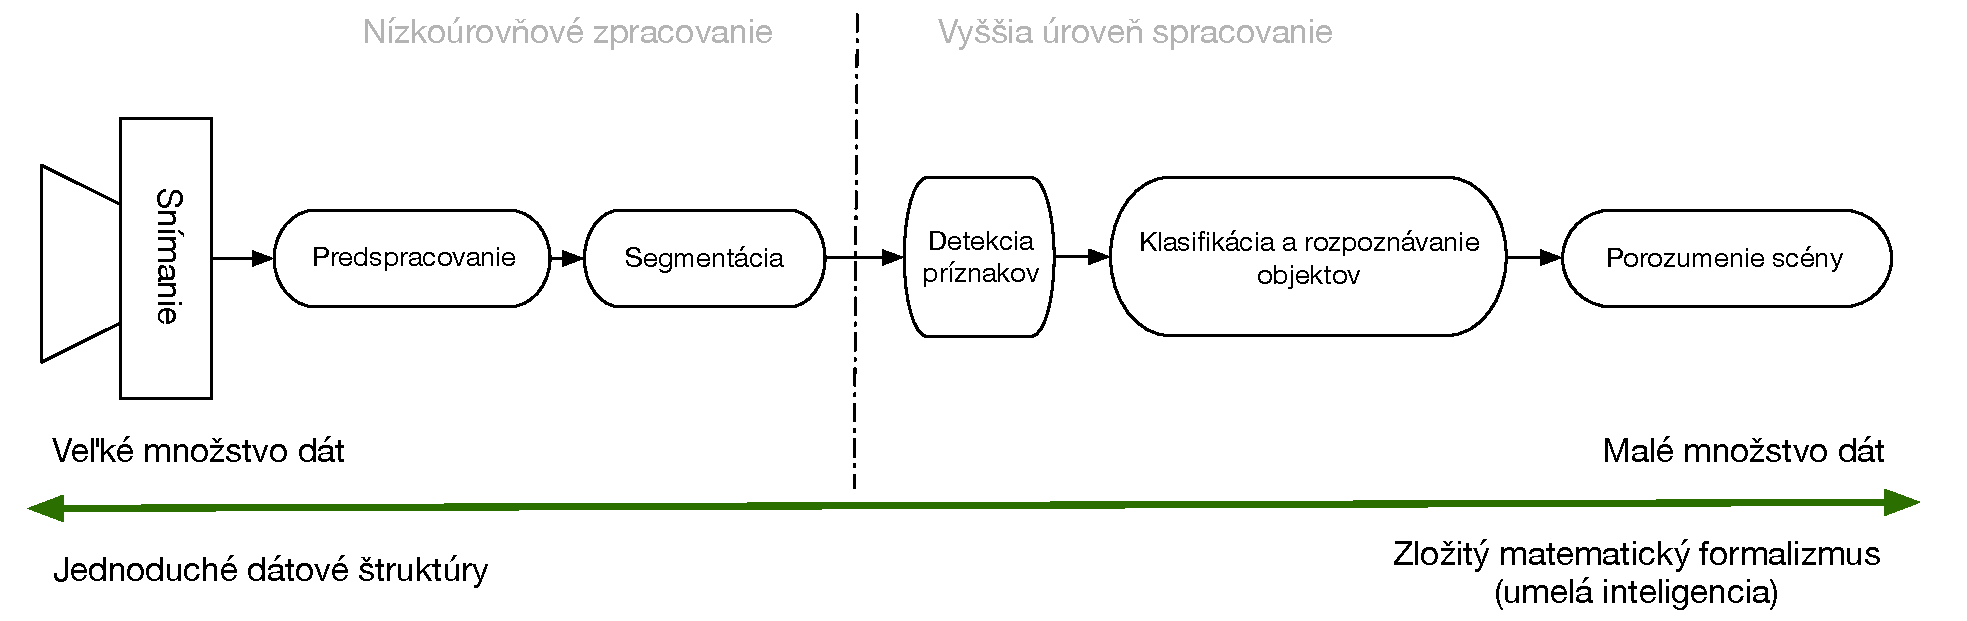
\includegraphics[scale=0.45]{obrazky/etapy}
	\caption{Etapy spracovania obrazu}
	\end{center}
\end{figure}

V nasledujúcom texte si postupne opíšeme každú fázu modelu. 


\subsection{Snímanie}
Základným obmedzením pri vnímaní okolitého 3D sveta, je skutočnosť, že človek dokáže vnímať okolie len 2D, ktorý predstavuje len zjednodušený model 3D okolia.


\subsubsection{Dierková komora}Tento model kamery možno použiť ako prvú aproximáciu mapovania 3D scény do 2D obrazu. Je to model kamery, možno ju použiť ako prvú aproximáciu mapovania 3D scény do 2D obrazu. Je to analógia toho, čo vzniká na sietnici ľudského oka. Obraz sa premieta do obrazovej roviny vzdialenej od dierky o ohniskovej vzdialenosti $f$. V prípade, že sa zrkadlová rovina presunie pred rovinu projekcie z podobnosti trojuholníkov vyplýva tento vzorec:

\begin{figure}[H]
\begin{left}
	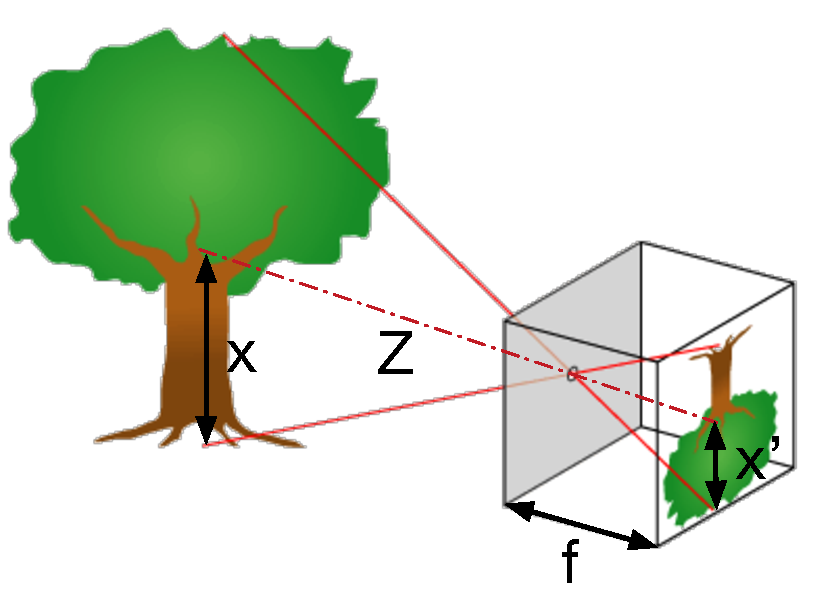
\includegraphics[scale=0.4]{obrazky/dierkovaKamera}
	\caption{Vyvolanie a prebeh zmeny stavu v komponente}
	\end{left}
\end{figure}

$$\textit{x}=\frac{X\textit{f}}{Z}$$

Tento výraz predstavuje najjednoduchší model dierkovej kamery, ktorý je základom zložitejších modelov slúžiacich na výpočty napr. pri 3D projekcií. 

\subsubsection{Prevedenie obrazu do počítača (snímanie)}
Je proces transformácie fyzikálneho obrazu do podoby vhodne pre spracovanie za pomoci počítača (matica pixlov). Tento proces sa skladá z troch častí: 
\begin{itemize}
\item \textbf{Snímanie} (scaning) - Cieľom prvého kroku je prevod optických veličín na elektrické. Pri použití nekvalitného snímača sa na výstupe objaví veľké množstvo šumu, ktoré len ťažko možno korigovať. Preto je nutné dbať na zaistenie čo najväčšej kvality snímača. 

\item \textbf{Vzorkovanie} - Shanonova veta i vzorkovaní nám vraví, že vzorkovacia frekvencia musí byť aspoň 2x väčšia než je maximálna frekvencia, ktorú obsahuje vzorkovací signál.
$$\textit{f}_{\textit{vzor}} \ge {2} \textit{f}_{\textit{max}}$$

V obrazovej terminológii nám táto veta vraví, že interval vzorkovania musí byť menší alebo rovný polovici rozmerov najmenších detailov na obraze. 

\item \textbf{Kvantovanie} 
Kvantovanie je prevod hodnoty obrazovej funkcie do číselnej hodnoty. Vždy je to proces stratový a nevratný. Počet kvantovacích bodov musí byť dostatočne jemný. Najčastejšie sa v praxi používa 256 úrovní jasu, čo vieme zakódovať do 8 bitov. Výnimku tvoria binárne obrazy, ktoré si vystačia len s dvoma úrovňami 0 a 1. Často sa používa na vytvorenie masky v ktorej možno ľahko nájsť kontúry. Najväčší problém kvantovania na nedostatočný počet úrovní je vnímanie falošných hrán. Možno odstrániť nelineárnym kvantovaním, alebo rozostrením obrazu. 



\item \textbf{Dátové štruktúry} - Najčastejšou reprezentáciu celého obrazu je \textbf{matica} hodnôt. Súradnice prvku v matice zodpovedajú súradniciam pixlu na obraze. Jeho hodnota zodpovedá napríklad jasu.  Okrem nej sa však používajú aj iné ako napríklad kódovanie kontúr segmentovaných objektov. Kontúra je uzavretá hranica objektu, ktorá môže reprezentovať objekt reálneho sveta na obraze a môže byť zdrojom informácii o ňom (tvar, farba, veľkosť).

Ďalšou možnosťou kódovania je \textbf{Run-length coding} forma reťazového kódu, použitá hlavne v binárnych obrazoch. 

\textbf{Freemanov (reťazový) kód}  je určený počiatočným bodom a postupnosťou symbolov zodpovedajúcich úsečkám jednotkovej dĺžky v niekoľkých vopred stanovených orientáciách. 

\textbf{Polygonálna reprezentácia hranice} je reprezentácia, ktorá aproximuje oblasť mnohouholníkom. Každá hranica je jednoznačne určená vrcholmi aproximovaného mnohouholníka.

\textbf{Hierarchické dátové štruktúry} obsahuje okrem originálneho obrazu aj jeho zjednodušené časti. Typicky tieto dátové štruktúry pomáhajú znižovať výpočtovú náročnosť a to tak, že sa algoritmus najprv pustí na hrubšiu aproximáciu obrazu, kde sa vytipujú záujmové oblasti a ďalej sa algoritmus aplikuje už len na vybrané časti originálneho obrazu. Základné hierarchické reprezentácie sú pyramídy a kvadrantové stromy. 

\end{itemize}



\subsection{Predspracovanie obrazu}
Vstupom aj výstupom je obraz na nízkej úrovni abstrakcie. Slúži na zlepšenie obrazu z hadiska ďalšieho spracovania. Môže potlačiť alebo naopak zvýrazniť isté informácie v obraze. Metódy spracovania delíme na: 
\begin{itemize}
\item Bodové jasové transformácie
\item Geometrické transformácie
\item Lokálne predspracovanie (filtrácia, ostrenie a detekcia hrán)
\item Obnovenie obrazu pri známej degradácii 
\item Matematická morfológia 
\end{itemize}

\subsubsection{Bodové jasové transformácie}

\textit{Jasová korekcia} - Používa sa pri nerovnomernom osvetlení obrazu. Pokiaľ je porucha
osvetlenia systematická, vieme korigovať odchýlku každého bodu od ideálnej charakteristiky.

\textit{Modifikácia jasovej stupnice} - Na rozdiel od jasovej korekcie, modifikácia stupnice nezávisí na polohe bodu v obraze. Táto modifikácia $T$ prevedie vstupnú jasovú hodnotu na výstupnú a to pomocou známej funkcie (tabuľky). 


\subsubsection{Geometrické transformácie}
Geometrická transformácia 2D obrazu je vektorová transformácia $T$, ktorá zobrazí bod ($x$,$y$) do bodu ($x_0$, $y_0$).  Jedná sa teda o transformáciu súradníc bodov obrazu. Vďaka tomu môžeme odstrániť geometrické skreslenie vzniknuté pri snímaní obrazu (napr. korekcie geometrických porúch objektívu kamery, oprava skreslenia družicového snímku spôsobená zakrivením zemegule).  Z toho vyplýva, že pomocou referenčnej mriežky vieme vyrovnať geometricky deformovaný obraz. Transformačné rovnice môžu byť známe alebo odvodené na základe vstupného a transformačného  obrazu. Pred začiatkom transformácie sa musia nájsť dvojice zodpovedajúcich si bodov (vlícovacie body), ktoré sa na obrázkoch ľahko hľadajú napr. priesečníky vláknitých štruktúr, rohy objektov a pod. Následne sa vykoná transformácia súradníc bodov do nových pozícii. A nakoniec sa musí vykonať aproximácia jasovej funkcie.

\begin{figure}[H]
\begin{center}
	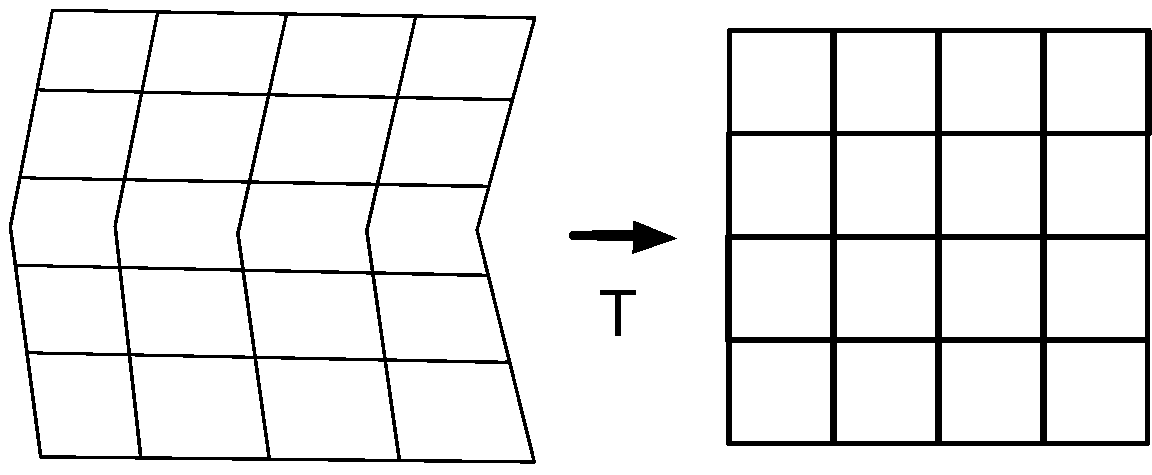
\includegraphics[scale=0.4]{obrazky/geometrickaTransformacia}
	\caption{Príklad geometrickej transformácie}
	\end{center}
\end{figure}

\subsubsection{Lokálne predspracovanie - filtrácia}
Používa sa na odstránenie vysokofrekvenčných zložiek, čo predstavujú hrany a šum. Pri tejto operácii dochádza k stratení detailov obrazu (rozmazanie).

\textit{Spriemerovanie} - Ide o najjednoduchší prostriedok pre vyhladenie šumu v obraze. Pre každý bod obrazu sa jeho jas nahradí aritmetickým priemerov jasov jeho susedov. Filtrácia spriemerovaním je vlastne špeciálny prípad konvolúcie, kde konvolučná maska vyzerá nasledovne:
$$\textit{h}=\frac{1}{9}\begin{bmatrix} 1 & 1 & 1 \\ 1 & 1 & 1 \\ 1 & 1 & 1  \end{bmatrix}$$

\textit{Filtrovanie pomocou Gaussovej masky} - Gaussovú masku dostaneme posilnením stredového bodu, prípadne jeho štyroch susedov, tak aby lepšie aproximoval šum s Gaussovým rozdelením.
$$\textit{h}=\frac{1}{10}\begin{bmatrix} 1 & 1 & 1 \\ 1 & 2 & 1 \\ 1 & 1 & 1  \end{bmatrix}$$
$$\textit{h}=\frac{1}{16}\begin{bmatrix} 1 & 2 & 1 \\ 2 & 4 & 2 \\ 1 & 2 & 1  \end{bmatrix}$$

\textit{Mediánový filter} - Medián alebo prostredná hodnota je hodnota, ktorá rozdeľuje postupnosť podľa veľkosti zoradených výsledkov na dve rovnako početné polovice. V štatistike patrí medzi stredné hodnoty. Usporiadame jasové úrovne z lokálneho okolia a vyberieme strednú hodnotu usporiadania. To zabráni, aby krajné extrémy ovplyvnili vybranú hodnotu. Filtrácia však nieje vhodná v obraze, kde sa nachádzajú tenké čiary a ostré rohy. 


\subsubsection{Lokálne predspracovanie - Detekcia hrán}
Opak filtrácie, zvyšuje vysokofrekvenčné časti spektra (hrán) a odstránenie nízkofrekvenčných častí. Sprievodný javom je aj zvýraznenie šumu v obraze.  Hrana je vektorová veličina, určená veľkostnou a smerom. Pri hranovej detekcii sa využíva vlastnosť gradientu,ktorá hovorí, že hodnota gradientu funkcie dvoch premenných je v oblasti hrany najväčšia. 

\textit{Laplacov operátor} - Tento operátor aproximuje druhú deriváciu a predstavuje rýchlosť zmeny hodnôt jasu. Prejaví sa najmä na strmých alebo izolovaných hranách alebo ju možno použiť na detekciu izolovaných bodov. Bude zvýrazňovať aj šum.
$$\textit{h}_1=\begin{bmatrix} 0 & 1 & 0 \\ 1 & -4 & 1 \\ 0 & 1 & 0  \end{bmatrix}$$
$$\textit{h}=\begin{bmatrix} 0 & 0 & -1 & 0 & 0 \\ 0 & -1 & -2 & -1 & 0 \\ -1 & -2 & 16 & -2 & -1 \\ 0 & -1 & -2 & -1 & 0 \\ 0 & 0 & -1 & 0 & 0  \end{bmatrix}$$
Spolu s Laplaceovým operátorom sa používa i vyhladzovací Gaussovnský filter. Vtedy hovoríme o Laplaciáne Gaussiánu – LoG (matica $h$).

\textit{Sobelov operátor} - Aproximuje prvé parciálne derivácie. Nakoľko samotná derivácia zvýrazňuje šum, vykonáva ja vyhladzovanie. Pre každý smer hrán existuje špeciálna maska.
$$\textit{h}_1=\begin{bmatrix} 1 & 2 & 1 \\ 0 & 0 & 0 \\ -1 & -2 & -1  \end{bmatrix}$$
$$\textit{h}_2=\begin{bmatrix} 0 & 1 & 2 \\ -1 & 0 & 1 \\ -2 & -1 & 0  \end{bmatrix}$$

\begin{figure}[H]
\begin{center}
	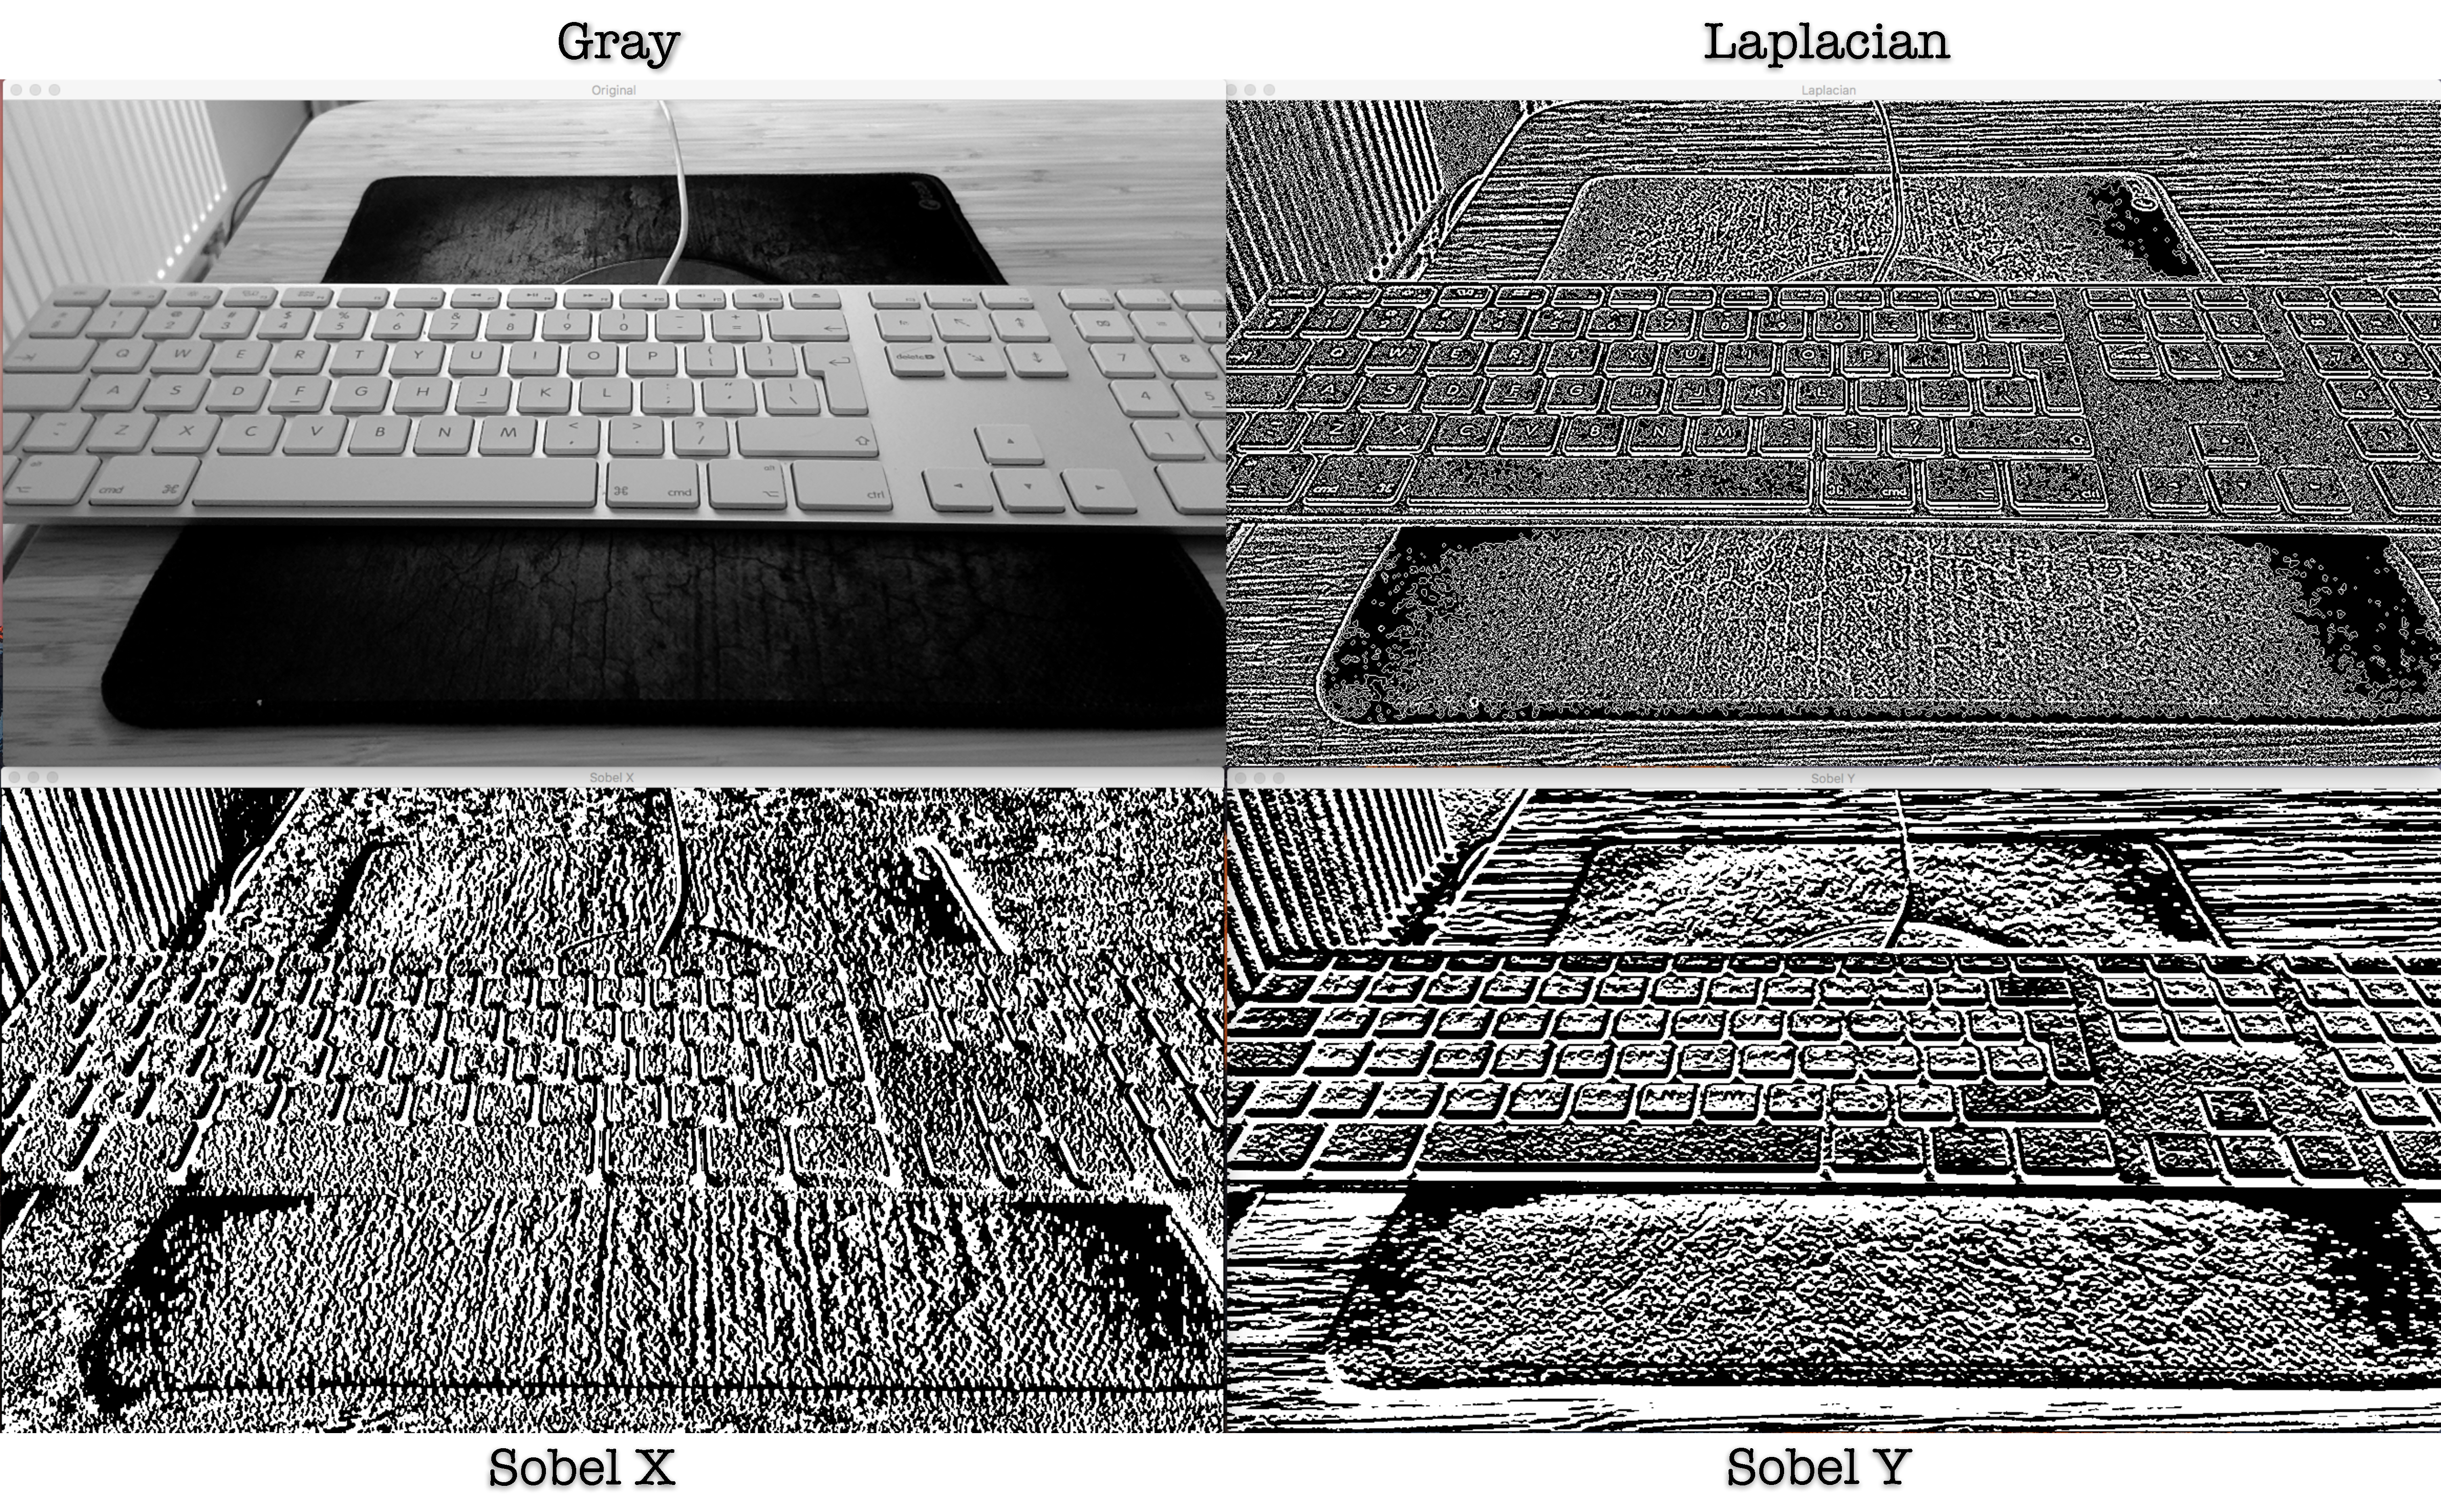
\includegraphics[scale=0.16]{obrazky/hranove_filtre}
	\caption{Vzájomné porovnanie algoritmou pre detekciu hrán}
	\end{center}
\end{figure}


\subsection{Segmentácia obrazu}
Segmentácia je rozdelenie obrázku na časti, ktoré silne korelujú s objektami reálneho sveta. Pri čiastočnej segmentácii je cieľom rozdeliť obraz na časti, ktoré sú homogénne z hľadiska vybranej vlastnosti (farba, jas, odrazivosť atď …) Cieľom segmentácií v počítačovom videní je značná redukcia objemu dát. Nejednoznačnosť obrazových dát je hlavným problémom segmentačného procesu. Segmentačné metódy možno rozdeliť na tri skupiny: 


\begin{itemize}
\item Prahovanie
\item Segmentácia založená na hranách (diskontinuita)
\item Segmentácia založená na oblastiach (podobnosť)
\end{itemize}

\subsubsection{Prahovanie}
Najjednoduchšia segmentačná technika. Je založená na predpoklade, že jednotlivé objekty majú konštantnú obrazivosť, či pohltivosť svetla na svojom povrchu. Je to transformácia, ktorá zobrazuje vstupný obraz $f(i, j)$ na výstupný obraz $g(i, j)$ nasledovne: 
$$g (i{,}j)=1 {,}\quad {ak} f(i{,}j)\ge T$$
$$g (i{,}j)=0 {,}\quad {ak} f(i{,}j)  < T$$


Z toho vyplýva, že na segmentovanie objektov od pozadia sa používa jasová konštanta, ktorá sa nazýva prah. 


\textit{Globálne prahovanie} - Je to technika. ktorá je vhodná, keď sa objekty na scéne diametrálne líšia svojimi charakteristikami. V takom prípade môžeme nastaviť prah ako interval platných hodnôt. Príklad použitia môžeme vidieť na obrázku s kačkou. Originálny obrázok sa konvertuje do HSV farebného priestoru, ktorý umožňuje lepšiu prácu s odtieňmi farieb spôsobené nehomogénnym osvetlením. Následne sa aplikuje filter ktorý prepustí len hodnoty v danom intervale.

\begin{figure}[H]
\begin{center}
	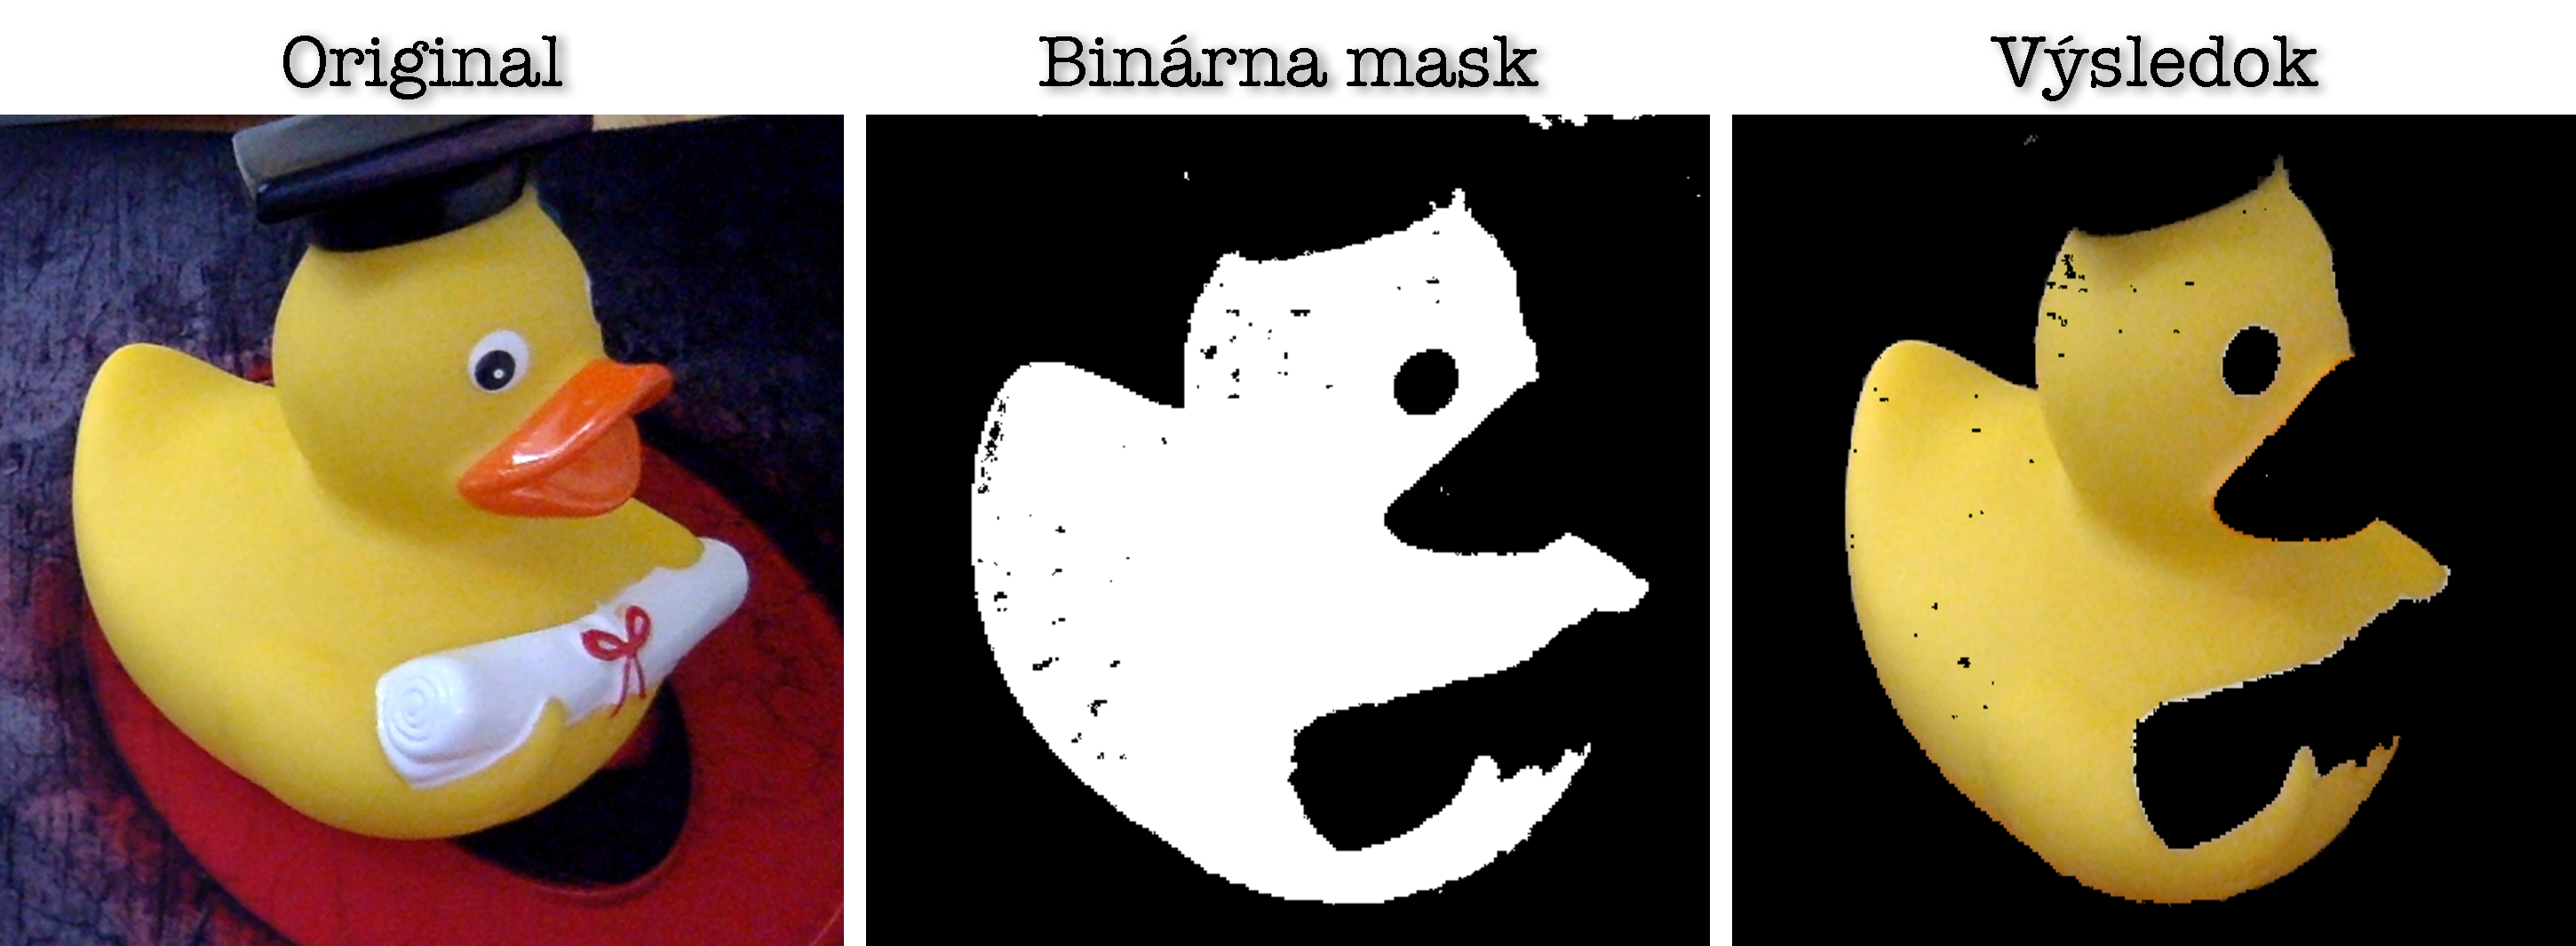
\includegraphics[scale=0.25]{obrazky/prahovanie}
	\caption{Detekcia tela kačky na základe prahovania}
	\end{center}
\end{figure}


\textit{Lokálne prahovanie} - Málokedy je možné použiť jednu hodnotu prahu (alebo interval) na celý obraz, z dôvodu fyzikálnym podobnostiam objektov v scéne a  nehomogénnemu osvetleniu scény. Preto sa často používajú metódy lokálneho prahovania. Algoritmy sa počítajú v malých regiónoch obrazu. Tak dostaneme rôzne prahové hodnoty pre rôzne regióny rovnakého obrazu a to nám dáva lepšie výsledky u snímok s rôznym osvetlením. Môžeme ho definovať takto : 
$$T=T(f {,} f_c){,}$$

kde $f_c$ je časť obrazu v ktorej sa určuje prah. 

\begin{figure}[H]
\begin{center}
	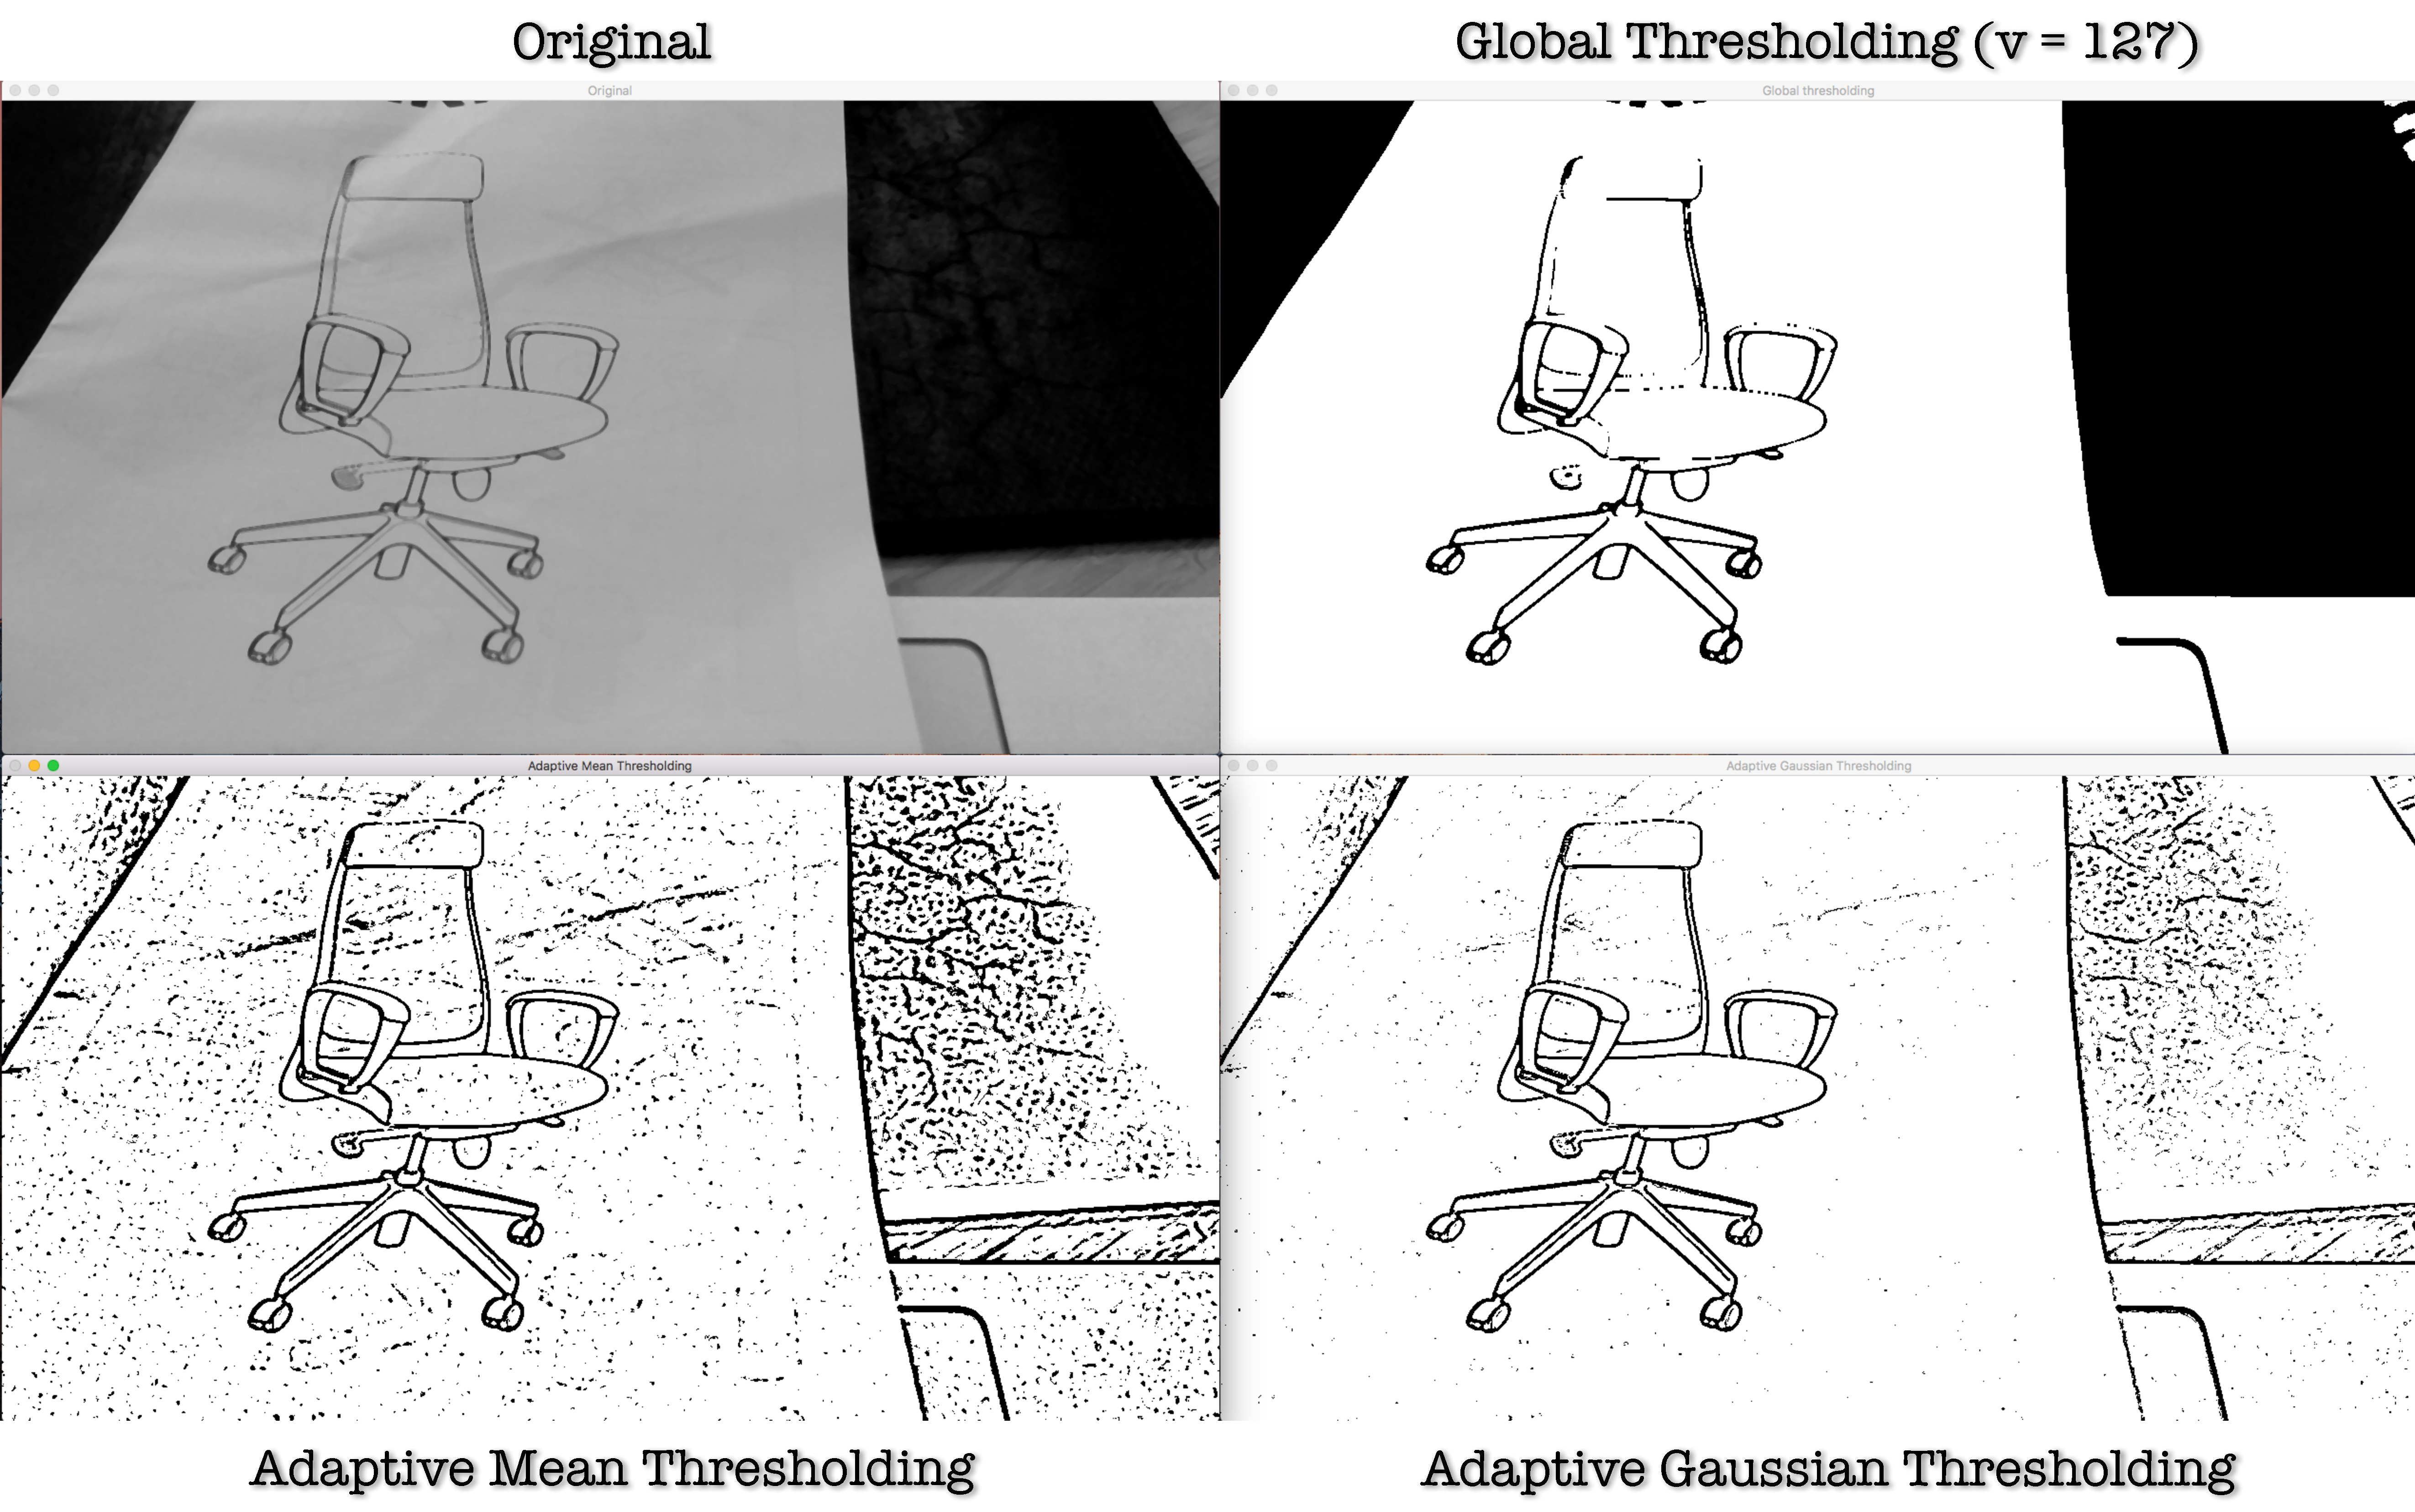
\includegraphics[scale=0.15]{obrazky/lokalne_prahovanie}
	\caption{Porovnanie výsledkov metod lokalneho prahovania}
	\end{center}
\end{figure}



\subsubsection{Segmentácia na základe detekcie hrán}
Techniky založené na informáciach, ktoré poskytujú hrany v obraze. Preto je  nutné si vysvetliť aký rozdiel je medzi pojmom hrana a hranica. Hrana je miesto kde sa skokovito mení hodnota obrazovej funkcie. Pre účely segmentácie sú však dôležitejšie hranice regiónov.  Región je množina súvislých bodov a hranicu regiónu je množinu bodov, ktoré sú súčasťou regiónu, ale zároveň aspoň jeden z ich susedov nepatri regiónu. Takáto hranica tvorí vnútornú hranicu regiónu. 

\textbf{Metóda sledovania hranice}
Táto metóda pracuje na binárnom obraze. Vnútornú hranicu získame tak, že  prehľadávame obraz zľava doprava, zhora dole, pokiaľ nenarazíme na bod patriaci regiónu. Tento bod pridáme do hranice. Nasledovne prehľadávame okolie tohoto bodu v protismere hodinových ručičiek od posledne navštíveného bodu. Pokiaľ narazíme na bod, ktorý je patriaci do rovnakého regiónu, pridáme ho do hranice. Tento postup opakujeme dokiaľ sa nedostaneme naspäť k počiatočnému bodu. 

Algoritmus nájde iba vnútorne hranice. Pokiaľ chcem nájsť vonkajšie hranice, môžeme ich získať tak že, nájdeme vnútorné. Potom vonkajšiu hranicu tvoria body, ktoré sme pri vyhľadávaní vnútornej hranice testovali, ale nepatrili do regiónu. 

Tento algoritmus funguje pre oblasti väčšie než 1 pixel.  Ide o veľmi obľúbený a účinný algoritmus, ktorý sa veľmi často používa.

\textbf{Cannyho detektor}
Jeden z najlepších a najpoužívanejších algoritmov pre detekciu hrán, ktorý je založený na hľadaní hodnoty gradientu a spoľahlivosti bodu na základe susedných bodoch. Požiadavky na úspešnosť sú presnosť, minimálny počet chýb a jednoznačnosť. 

Prvý krok algoritmu je eliminácia šumu použitím \textit{Gaussovho filtra}.  Následne nájdeme miesto a smer gradientu použitím \textit{Sobelového operátora}. Ďalej musíme odobrať z hodnôt gradientu  body, ktoré nie sú lokálne maximá. Napríklad, ak máme pixel, ktorým prechádza zvislá hrana, musí byť jeho ľavý a pravý sused nižšej hodnoty, aby bol uznaný  ako skutočná hrana. V poslednom kroku musíme uplatniť metódu \textit{prahovania s hysteréziou}. Zvolíme si minimálny (T1) a maximálny (T2) prah medzi ktorým môže gradient kolísať.  Ak je hodnota gradientu pixlu vyššia než T2 je pixel označený ako hranový. Ak hodnota bodu leží medzi T1 a T2 bod je uznaný ako hranový len vtedy, ak leží vedľa suseda označeného ako hranový.


\textbf{Hľadanie hraníc Houghovou transformáciou}
Pomocou tejto metódy je možné nájsť v obraze objekt, ktorého tvar je možné popísať analytickým výrazom (priamka, kruh, elipsa …). Veľkou výhodou je invariantnosť metódy na zmenu mierky, pootočenie a veľká odolnosť voči pôsobeniu šumu v obraze. 

\subsubsection{Segmentácia založená na spájaní a delení oblastí}
Metódy tejto kategórie nehľadajú hranice jednotlivých regiónov ale snažia sa o nájdenie oblastí priamo. Hlavná myšlienka je založená na klasifikácii obrazu do niekoľkých spojitých homogénnych podoblastí, ktoré sú vzájomne disjunktné, pričom zjednotením podoblastí je celý obraz.
$$R=\bigcup_{i=1}^s R_i{,}\quad R_i\bigcap R_j=0{,}\quad{pre}\quad i\neq j$$

Medzi základné podmienky segmentácie patrí kritérium homogenity:
$$H(R_i)={THRUE}{,}\quad \textit{i}=1{,}2{,}{...}{,}s{,}$$
$$H(R_i \cup R_j)={FALSE}{,}\quad \textit{i} \neq \textit{j}{,}\quad R_i { \ je \ susedné \ k \ } R_j $$

kde S je celkový počet regiónov v obraze a $H(R_i)$ je hodnota binárne homogenity regiónu $R_i$. Prvá podmienka sa týka vlastností, ktoré musia spĺňať pixle v segmentovanom regióne, druhá určuje, že susedné regióny $R_i$ a $R_j$ majú odlišné veľkosti. Existuje veľké množstvo metód založených na segmentácii regiónov, pričom sa z výkonnostného hľadiska veľmi nelíšia. Veľkou výhodou metód tejto kategórie je odolnosť voči šumu, preto v prípadoch veľkého zašumenia obrazu sú lepšou cestou oproti metódam založených na detekcii hrán avšak na úkor väčšej výpočtovej náročnosti.  

\subsection{Príznaky a rozpoznávanie}
Proces segmentácie zaručuje, že obraz bol rozdelený do vzájomne disjunktných častí. To však vo väčšine prípadov nestačí a je nutné rozdeliť jednotlivé regióny tak, aby korelovali s objektami reálneho sveta. To si však vyžaduje vytvoriť exaktný popis oblastí. Až na základe neho môže klasifikátor rozdeliť jednotlivé objekty do tried.  Z toho vyplýva, že proces segmentácie bezprostredne predchádza procesu klasifikácie.  Tento proces však nieje vždy nutný. Ak je cieľom odlíšenie objektov od pozadia výsledkom takejto snahy je binárny obraz, kde objekty záujmu sú biele a nepodstatné okolie čierne.
Rozpoznávanie je klasifikačná úloha. Existujú dve základné formy opisu objektu, podľa nich delíme aj metódy rozpoznávania na dve základné skupiny: 

\begin{itemize}
\item Príznakové - príznaky popisujúce objekt 
\item Syntaktické - pomocou primitív (formálne gramatiky, produkčné pravidlá, fuzzy logika)
\end{itemize}

\subsubsection{Skalárne deskriptory}
Je to výsledok merania ktorý kvantifikuje nejakú vlastnosť. Medzi jednoduché skalárne deskriptory  patria napríklad veľkosť,  okrúhlosť, obvod dĺžka hlavnej osi, uhol hlavnej osi, ťažisko,  projekcia, výška, šírka, výstrednosť, pozdĺžnosť, pravouhlosť, smer, nekompaktnosť, Feretov priemer a iné. 

Tvarové invarianty. Sú to deskriptory tvaru objektu, ktoré sú invariantné k určitej triede transformácii.
Často používané sú aj viacrozmerné skalárne deskriptory medzi ktoré patrí napríklad obraz, histogram alebo kombinácia skalárnych deskriptorov.

\subsubsection{Momenty}

Jeho všeobecná definícia je takáto:
$$m_{pq}=\sum_{i=\infty}^\infty \sum_{i=\infty}^\infty i^p j^q f(j,j)$$
Na základe momentov je možné vypočítať charakteristiky oblastí, ako napríklad ťažisko takto: 
$$x_c=\frac{m_{10}}{m_{00}}\ {,}\quad y_c=\frac{m_{01}}{m_{00}}$$
Následne je možné definovať centrálny moment, ktorý je invariantný voči posunu. 


\subsubsection{Štatistické metódy rozoznávania}
Tieto metódy úzko súvisia s pojmom klasifikácia a ich základom sú štatistické postupy. Klasifikátor je nástroj, ktorý na základe príznakov zaradí objekty do tried. Funkcie, ktoré oddeľujú jednotlivé triedy sú diskriminačné funkcie. Pokiaľ ich vieme znázorniť ako priamku, ide o lineárne klasifikároty. Existujú tri typy klasifikátorov: 

\begin{itemize}
\item Deterministický  – Založený na diskriminačných funkciách, určitá vzorka je vždy zaradená do určitej triedy 
\item Stochastický -  Založený na pravdepodobnosti, že klasifikátor zaradí niektorý z objektov do nesprávnej triedy (každé rozhodnutie nesie riziko chyby).  Napríklad Bazesov klasifikátor
\item Heuristický - neurónové siete, k-najbližších susedov, logistická regresia, Support Vector 
Machines (SVM), rozhodovacie stromy (Decision trees) 
\end{itemize}

\subsection{3D snímanie priestoru}
Základným princípom je projekcia lúčov odrazených od 3D objektov sveta na 2D plochu snímača. Pri tomto procese však dochádza k rôznym efektom pri ktorých sa stráca veľa informácii. Napríklad premietanie viacerých bodov 3D scény do jedného bodu na 2D senzore, prekrývanie objektov alebo aj šum. Existujú však metódy, ktorým sa darí dané problémy eliminovať a dosiahnuť tak  hlavný cieľ, ktorým je porozumieť 3D snímanej scéne. Metódy 3D snímania možno deliť do dvoch základných skupín: 

\begin{itemize}
\item Pasívne metódy
\item Aktívne metódy 
\end{itemize}

\subsubsection{Pasívne metódy - stereo videnie}
Tieto metódy potrebujú pre snímanie scény zisk z dvoch kamier zo vzájomne rôznou pozíciou a ľubovolným uhlom. 

\begin{figure}[H]
\begin{center}
	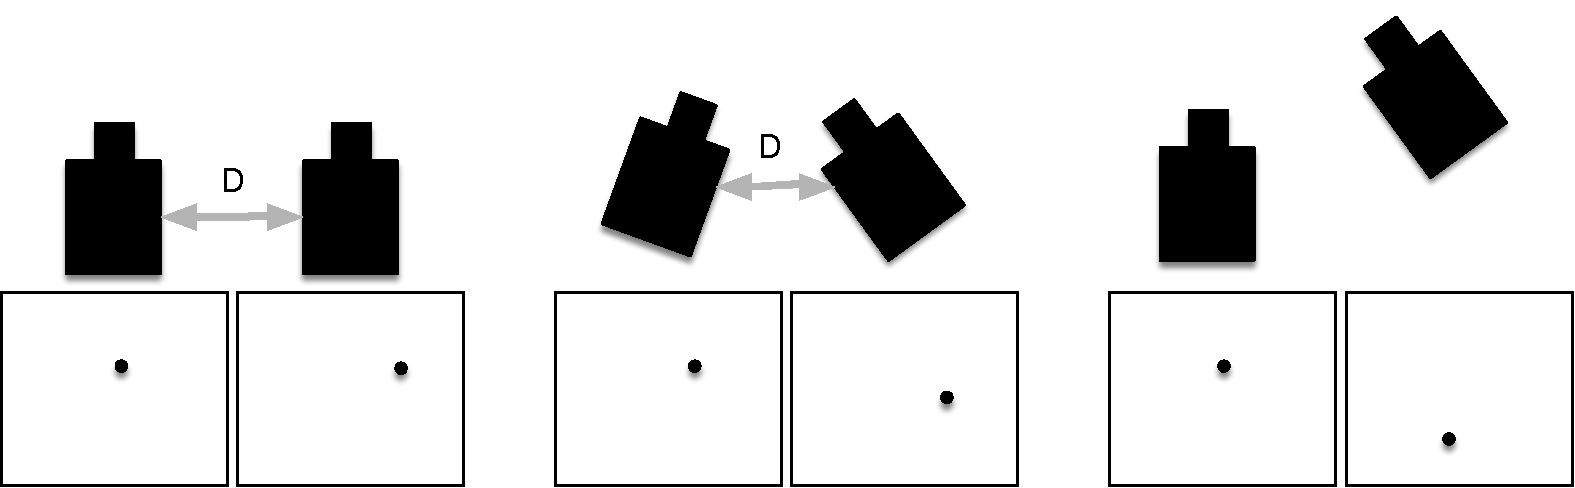
\includegraphics[scale=0.5]{obrazky/poloha_kamier_3D}
	\caption{Možnosti vzájomných polôch dvoch kamier}
	\end{center}
\end{figure}


V nasledujúcom texte sa však obmedzíme na situáciu A. Obe kamery snímajú scénu bod rovnakým uhlom a zo známou vzdialenostnou medi nimi. Táto situácia je rovnaká ako v ľudskom videní, len namiesto očí pracujeme s kamerami. Táto metóda je založená na triangulácii, čo je orientácia snímkovej dvojice. 

\begin{figure}[H]
\begin{center}
	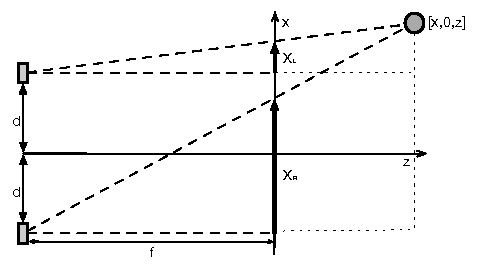
\includegraphics[scale=1.8]{obrazky/triangulacia}
	\caption{Výpočet vzdialenosti na základe tirangulácie}
	\end{center}
\end{figure}

podobnosti trojuholníkov potom platí:
$$\frac{X_L}{f}=\frac{x-d}{z}\ {;}\quad \frac{X_R}{f}\frac{x+d}{z}$$ 
$$ z=\frac{-2df}{X_L-X_R}$$

Z obrázka vyplýva, že pri známych veličinách $f$ (ohnisková vzdialenosť) a $d$ (vzdialenosť kamier od seba) vieme vypočítať pre každý pixel jeho hĺbku. Je to možné na základe disparity, čo je rozdiel medzi polohou bodu snímaného jednou kamerou oproti pozícii toho istého bodu snímaného druhov kamerou. Takže každý pixel scény pozorovanej dvoma kamerami má istú hodnotu disparity. Čim je vzdialenosť od kamier väčšia, tým je táto hodnota menšia a čím je vzdialenosť menšia hodnota disparity je väčšia. Implementácia je veľmi náročná. Vyžaduje si presné technické špecifikácie kamier a algoritmy, ktoré dokážu nájsť korešpondujúce body sú zložité. Najpoužívanejším je RANSAC. 

Pre kamery ktoré nie sú umiestnené v rektifikovanej  polohe sa používa epipolárna geometria. 


\subsubsection{Postupné ostrenie obrazu }
Pokiaľ máme k dispozícii kvalitnú kameru, ktorá dokáže selektívne zaostrovať na určitú vzdialenosť, vieme postupným procesom získať hĺbku každého pixlu, podľa momentu, kedy bol správne zaostrený. To, či je obraz na určitom mieste zaostrený, je možné určiť pomocou rôznych lokálnych operátorov známych z detektorov hrán (kapitola xxx). 


\subsubsection{Aktívna triangulácia }
Základným znakom je pridanie dodatočnej informácie do scény. Táto informácia môže byť reprezentovaná laserom, ifražiaričom alebo projektorom. Tieto metódy sa charakterizujú ako optické metódy merania vzdialenosti. Optické metódy sú také, ktoré meranie vykonávajú určitým optický lúčom.  Meranie je teda realizované postupným premietaním vzoru na predmet a následným zachytením kamerou. Podľa deformácie premietaného vzoru je možné následne určiť hĺbkovú mapu priestoru.

\subsection{Analýza pohybu }
Väčšina aplikácii, ktoré rieši počítačové videnie spočíva v nájdení, rozpoznaní a následnom sledovaní objektu, ktorý sa pohybuje po scéne. 

Veľmi používaná je detekcia samotného pohybu. V tomto druhu aplikácii statická kamera sleduje určitú scénu a je cieľom zistiť nežiadaný pohyb na sledovanej scéne. Ide o veľmi jednoduché aplikácie implementované napríklad aj v bezpečnostných kamerách ako inteligentná spúšť nahrávania.  Algoritmy nemajú za úlohu riešiť smer ani trajektóriu pohybu, sú schopné len vyrátať o koľko sa zmenila scéna oproti referenčnej vzorke. Jedna z najpoužívanejších metód je diferenčná metóda. Detekcia lokalizácia a predikcia pohybujúceho sa predmetu oproti detekcii samotného pohybu tieto metódy majú  za úlohu zistiť aj trajektóriu a vyrátať predikciu ďalšej polohy objektu. Medzi najkomplikovanejšie situácie patria tie, pri ktorých sa naraz môže pohybovať kamera ja objekt súčasne.

\subsubsection{Kalmanov filter}
Pri analýze pohybu objektu veľmi často dochádza k spájaniu, zatieneniu, či zmiznutiu sledovaného  objektu na obraze. Z toho dôvodu by sme potrebovali prostriedok, ktorý by spĺňal nasledovné podmienky: 


Očakávaná hodnota odhadu by mala byť rovná očakávanej hodnote stavu - Potrebujeme priemernú hodnotu odhadovaného stavu. Je nežiaduce aby odhadovaná hodnota bola posunutá nahor alebo nadol. 
Chceme nájsť taký prostriedok pre odhad, ktorý má čo najmenšiu variáciu chyby - odhadovaná a následne nameraná hodnota by sa mala líšiť minimálne. 



Všetky tieto predpoklady spĺňa práve Kalmanov filter, avšak je možné ho použiť len vtedy, ak  meraný systém je opísateľný iným lineárnym systémom. Je to z dôvodu aby Kalmanov filter nebol ovplyvnený šumom. Kalmanov filter teda hľadá najoptimálnejším odhad budúceho stavu na základe stavov minulých a popisu systému.  Existuje už vyše 50 rokov, no stále je jedným z najdôležitejším, a najodporučanejším algoritmom.

\begin{figure}[H]
\begin{center}
	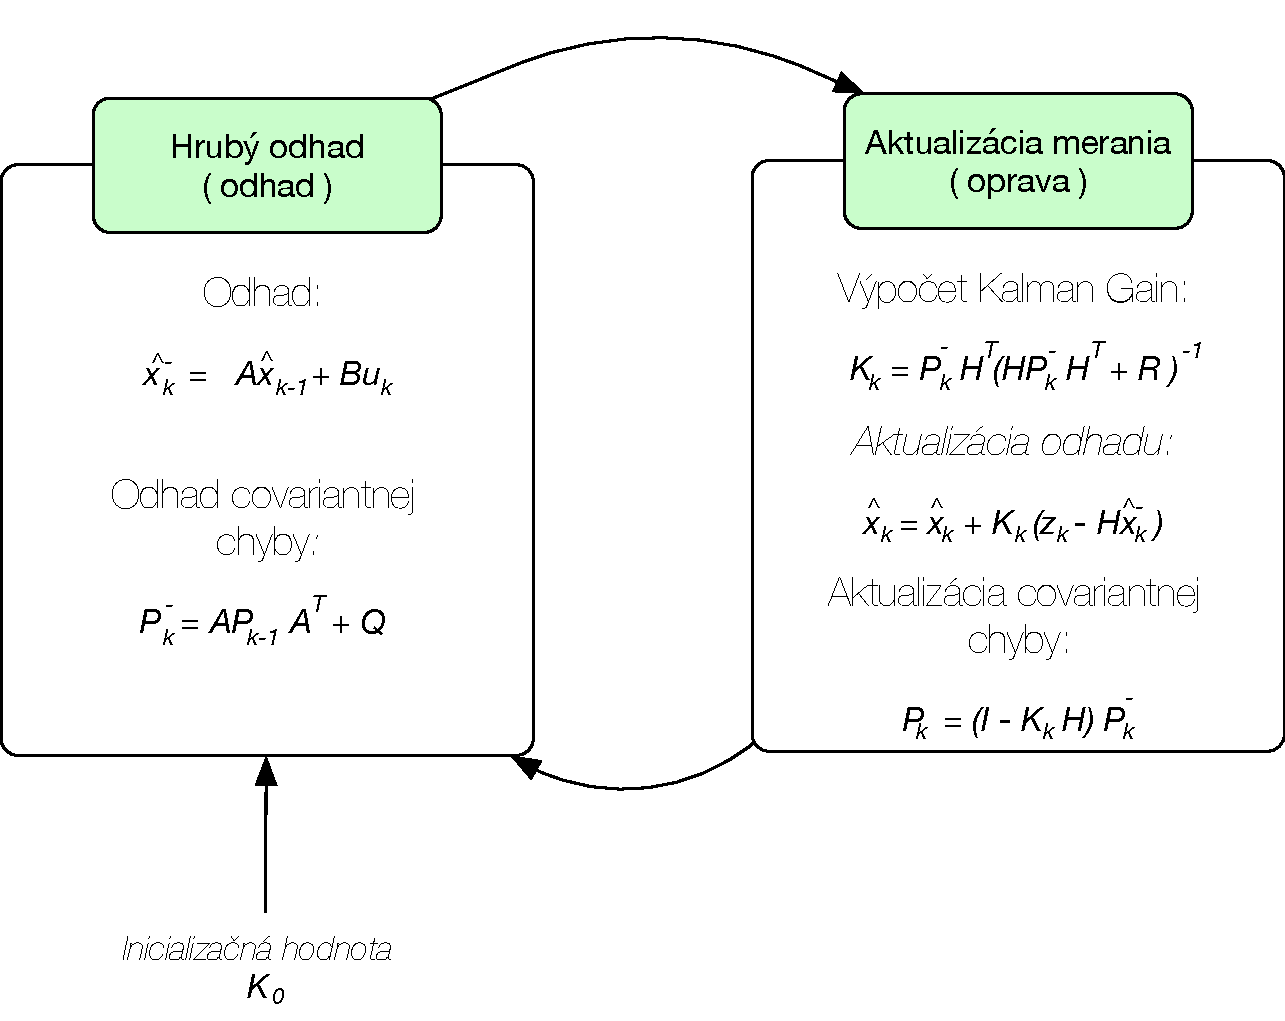
\includegraphics[scale=0.6]{obrazky/kalman}
	\caption{Popis algoritmu Klmanového filtra}
	\end{center}
\end{figure}

Hrubý odhad je predchádzajúci odhad polohy pred aktualizáciou merania. V časti aktualizácia merania už naozaj odhadneme nasledujúci krok. Z rovnice Kalman Gain alebo výpočet kalmanového zisku vyplýva, že ak je šum z merania R veľké, nebudeme dávať veľkú váhu meraniu pri výpočte ďalšieho kroku. Naopak ak je šum merania R malé, priradíme meranej hodnote veľkú váhu pri ďalšom kroku.  